\subsection{Máquina de cambios}
    \label{sec:switches}
 
    Una máquina de cambios (Figura \ref{fig:cambios_1}) es un mecanismo utilizado para permitir el paso de las formaciones de una vía a una ramificación del recorrido principal. Esto se realiza mediante el movimiento de la aguja del cambio (riel móvil) hacia su respectiva contraaguja (riel fijo) hasta obtener un adecuado acoplamiento que permita la circulación de la formación.

    \begin{figure}[H]
        \centering
        \includegraphics[width=0.9\textwidth]{Figuras/Cambios.jpg}
        \centering\caption{Máquina de cambios.}
        \label{fig:cambios_1}
    \end{figure}

    En la Figura \ref{fig:cambios_2} se muestra el cambio de vía de la estación Matheu de la Línea Mitre. Se observa que según sea la posición de la máquina de cambios, el tren puede continuar en la misma vía o hacer el cambio a la otra vía.

    \begin{figure}[H]
        \centering
        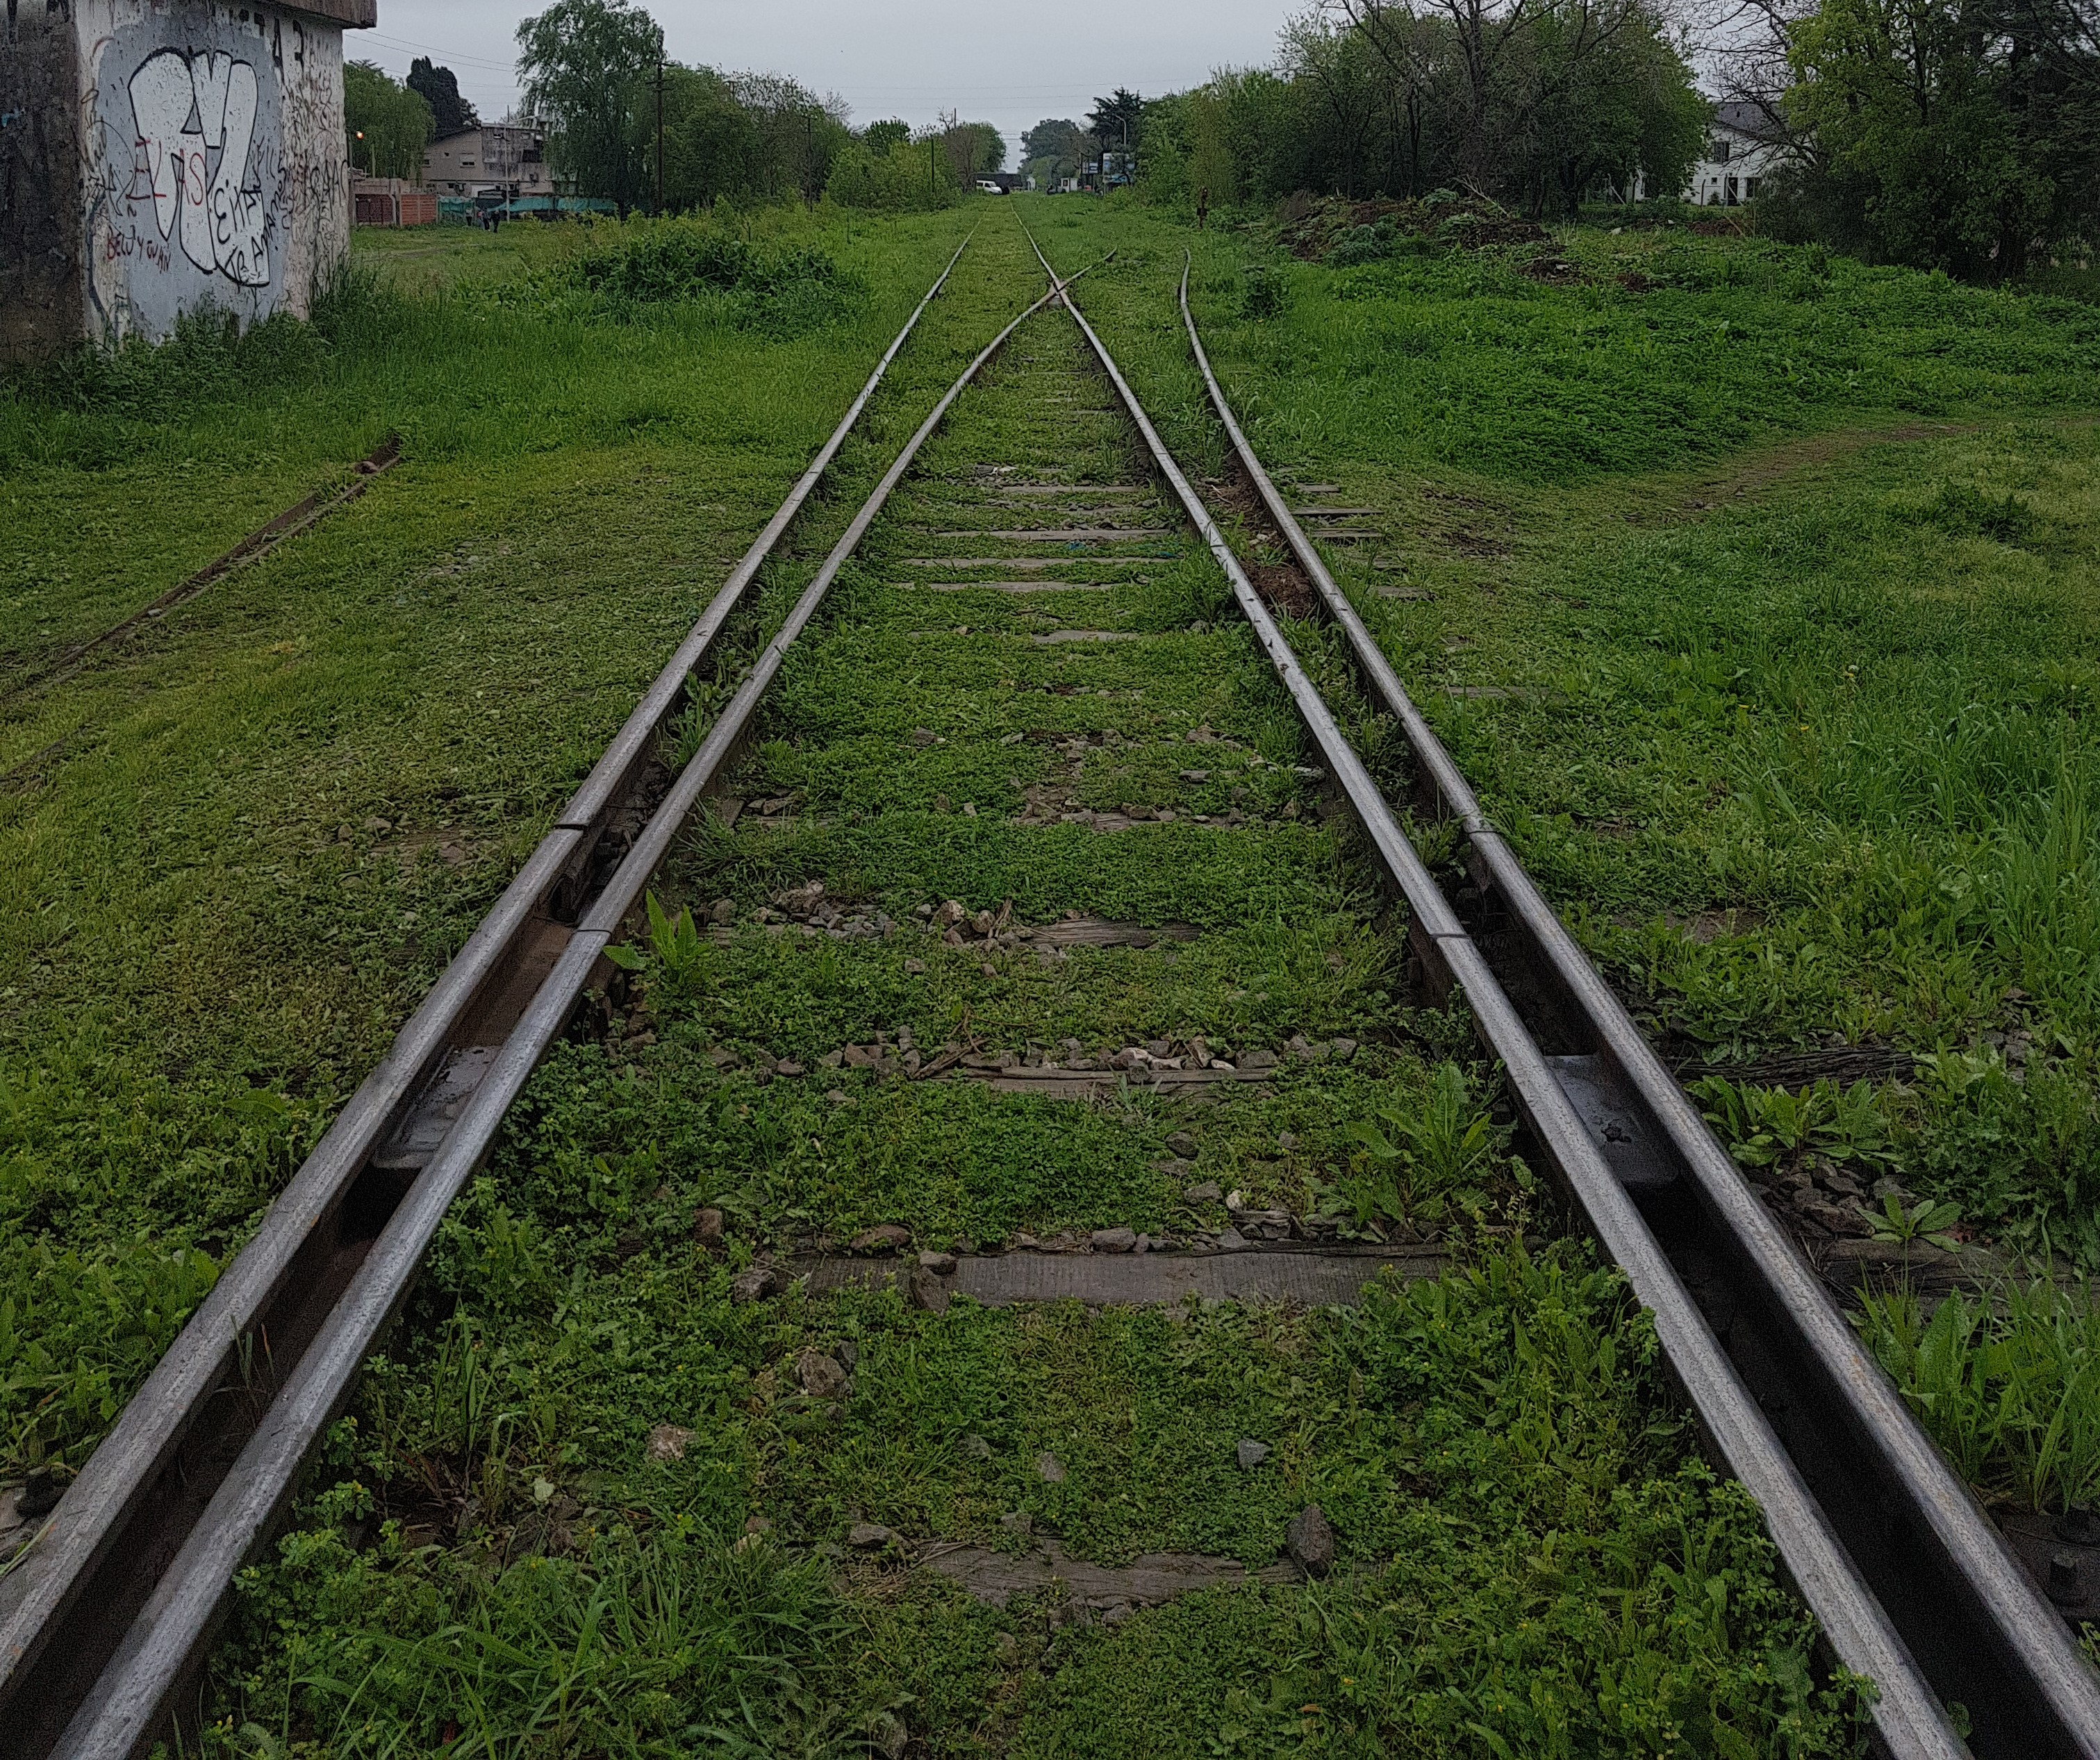
\includegraphics[width=0.9\textwidth]{Figuras/Cambios_2.jpg}
        \centering\caption{Cambio de vías de estación Matheu, Linea Mitre.}
        \label{fig:cambios_2}
    \end{figure}

    En la Figura \ref{fig:cambios_3} se muestran las posiciones que puede adoptar el cambio. En la posición normal, los trenes pueden circular de forma directa, en paralelo, por la vía principal en sentidos opuestos. En la posición reversa, en cambio, se permite el intercambio de trenes de una rama principal a otra en sentido opuesto o a una ramificación secundaria de la red.

    \begin{figure}[H]
        \centering
        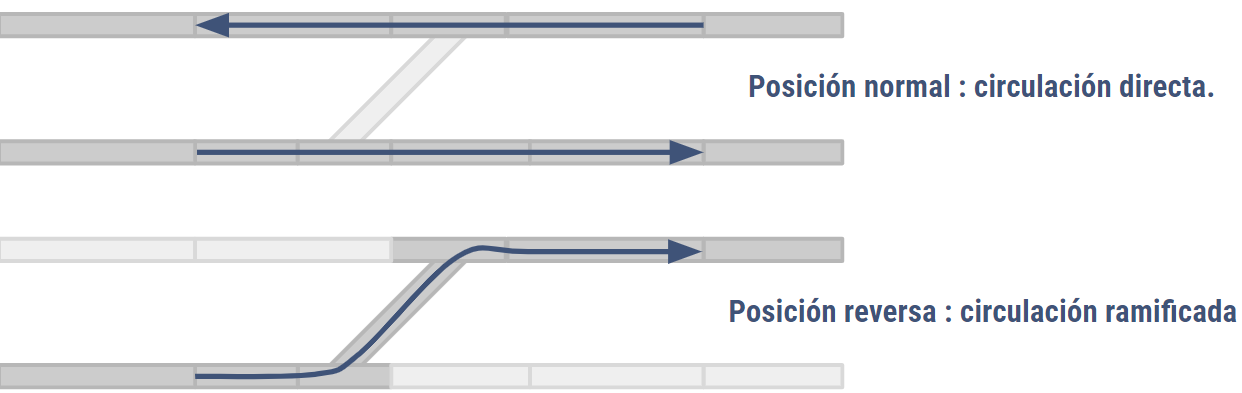
\includegraphics[width=0.9\textwidth]{Figuras/cambio_3.PNG}
        \centering\caption{Posiciones adoptadas por una máquina de cambios simple.}
        \label{fig:cambios_3}
    \end{figure}

    Las máquinas de cambios son un elemento activo de la red ferroviaria, controlados por el sistema de enclavamientos. Al ser mecanismos que necesitan tiempo para cambiar de un estado al otro, no puede asumirse que el comando es obedecido al instante. Incluso podría darse el caso que jamás llegue a cumplirse la orden debido a desperfectos mecánicos o eléctricos. Es por eso que introducimos los conceptos de comando, indicación y correspondencia, tal como se ilustran en la Figura \ref{fig:cambios_4}.

    \begin{figure}[H]
        \centering
        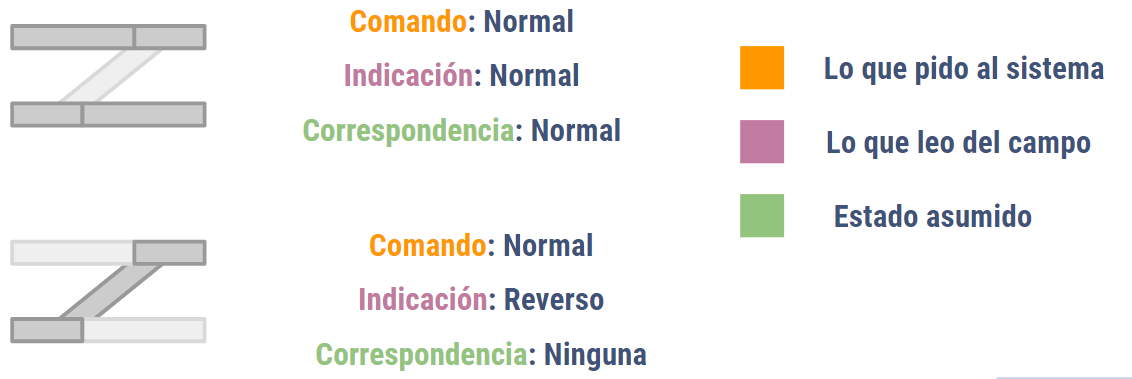
\includegraphics[width=1\textwidth]{Figuras/cambios}
        \centering\caption{Comando, indicación y correspondencia en máquinas de cambios.}
        \label{fig:cambios_4}
    \end{figure}
    
    El comando es la instrucción que el sistema de enclavamientos envía a la máquina de cambios. Esta instrucción puede ser modificar la posición de normal a reverso o de reverso a normal. La indicación es el estado que la máquina de cambios informa al sistema de enclavamientos. El sistema solo asume que el comando fue obedecido cuando tanto el comando como la indicación muestran una correspondencia. En caso contrario, el sistema de enclavamiento no puede asumir cual es el estado real del sistema, si el comando enviado o el estado reportado por la máquina de cambios. El mismo concepto puede ser aplicado en cualquier otro elemento mecánico, como por ejemplo las barreras ferroviarias.

    El RNA debe analizar diversos atributos distribuidos entre la clase switchIS (Código \ref{lst:switchIS}), la clase spotElementProjection (Código \ref{lst:switch}) y la clase switchIL (Código \ref{lst:switchIL}). La clase switchIS se encuentra dentro del vector de clases switchesIS, dentro de la clase functionalInfrastructure, que a su vez es parte de la clase infrastructure. La clase switchIS define el id de la máquina de cambios, el tipo (ordinario), el netElement al cual pertenece la entrada del cambio y hacia que lado se encuentra la vía de continuación y ramificación si transitamos desde el netElement del cambio hacia el cambio mismo. En este caso, si transitamos por el netElement ne16 el tren tendrá la vía de continuación en la mano derecha y la ramificación en la mano izquierda. Las máquina de cambio ordinarias siempre tienen una rama izquierda y una rama derecha definida. Además, dentro de la definición de cada rama tenemos el atributo netRelationRef, del cual se puede obtener, procesamiento mediante, los otros netElement correspondientes a las ramas: ne15 y ne14.

    \begin{lstlisting}[language = XML, caption = Clase switchIS switchIS , label = {lst:switchIS}]
    <switchIS id="swi84" continueCourse="right" branchCourse="left" type="ordinarySwitch">
        <name name="Sw01" language="en"/>
        <spotLocation id="swi84_sloc01" netElementRef="ne16" applicationDirection="reverse" intrinsicCoord="0.0000"/>
        <designator register="_Example" entry="SWITCH Sw01"/>
        <leftBranch netRelationRef="nr_ne15ne16_swi84" branchingSpeed="0" joiningSpeed="0" radius="-500"/>
        <rightBranch netRelationRef="nr_ne14ne16_swi84" branchingSpeed="0" joiningSpeed="0" radius="0"/>
    </switchIS>
    \end{lstlisting}

    La clase spotElementProjection define la ubicación en el espacio del elemento ferroviario referido. En este caso, como se puede ver en el Código \ref{lst:switch}, la posición de la máquina de cambios es la coordenada (-561 ; -450).

    \begin{lstlisting}[language = XML, caption = Clase spotElementProjection , label = {lst:switch}]
    <spotElementProjection refersToElement="swi84" id="vis01_sep16">
        <name name="Sw01" language="en"/>
        <coordinate x="-560.994" y="-450.000"/>
    </spotElementProjection>
    \end{lstlisting}

    La clase switchIL, definida dentro del vector de clases switchesIL, se encuentra dentro de la clase assetsForIL, en la clase interlocking. Contiene datos extra sobre el comportamiento dinámico de la máquina de cambios y define explícitamente los otros dos nodos, en contraposición a switchIS del cual hay que obtenerlos procesando un string. El RNA puede obtener los netElement de ambas clase y compararlos, anulando el análisis si los netElement definidos en switchIS y switchIL no son coincidentes.
    
    \begin{lstlisting}[language = XML, caption = Clase switchIL , label = {lst:switchIL}]
    <switchIL id="il_swi84" maxThrowTime="PT10S" typicalThrowTime="PT6S" isKeyLocked="false" returnsToPreferredPosition="false">
        <refersTo ref="swi84"/>
        <branchLeft ref="ne15"/>
        <branchRight ref="ne14"/>
    </switchIL>
    \end{lstlisting}
    
    El RNA utiliza el Algoritmo \ref{alg:switches} para detectar todos estos parámetros y crear un vector de máquinas de cambios (switches) indexado por el id de cada máquina de cambios (sw\_id). La existencia y ubicación de las máquinas de cambios ya se habían obtenido mediante el análisis de la red de grafos ferroviaria. El Algoritmo \ref{alg:switches} analiza la clase switchIS y confirma la existencia de la máquina de cambios, para luego la clase spotElementProjection y confirmar la ubicación de la misma. Los datos obtenidos en switches[sw\_id].LeftBranch y switches[sw\_id].RightBranch, permiten obtener los nodos de las ramificaciones que luego se conformarán analizando la clase switchIL en algoritmos posteriores.

    \begin{algorithm}[H]\captionsetup{labelfont={sc,bf}, labelsep=newline}
            \caption{Algoritmo detector de máquinas de cambios.}
            \label{alg:switches}
            \begin{algorithmic}
                \STATE \{switches\} $\gets$ \{\}
                \IF {infrastructure.SwitchesIS != None} 
                    \FOR{i in infrastructure.SwitchesIS[0].SwitchIS}
                        \IF{i.Id not in switchesIS.keys()}
                            \STATE sw\_id $\gets$ i.Name[0].Name
                            \STATE j $\gets$ i.SpotLocation[0]
                            \STATE left\_id $\gets$ i.LeftBranch[0].NetRelationRef
                            \STATE right\_id $\gets$ i.RightBranch[0].NetRelationRef
                            \STATE switches[sw\_id] $\gets$ \{"Node":j.NetElementRef\}
                            \STATE switches[sw\_id] $\gets$ \{"Continue":i.ContinueCourse\}
                            \STATE switches[sw\_id] $\gets$ \{"Branch":i.BranchCourse\}
                            \STATE switches[sw\_id] $\gets$ \{"Dir":j.ApplicationDirection\}
                            \STATE switches[sw\_id] $\gets$ \{"LeftBranch":j.left\_id\}
                            \STATE switches[sw\_id] $\gets$ \{"RightBranch":j.right\_id\}
                        \ENDIF
                    \ENDFOR
                \ENDIF
                \STATE visual\_data $\gets$ visualization.Visualization
                \IF {visual\_data != None}
                    \FOR {i in  visual\_data[0].SpotElementProjection}
                        \STATE sw\_id $\gets$ i.Name[0].Name
                        \IF {'Sw' in sw\_id}
                            \STATE pos\_x $\gets$ int(i.Coordinate[0].X)
                            \STATE pos\_y $\gets$ int(i.Coordinate[0].Y)
                            \STATE switches[sw\_id] $\gets$ \{"Position":[pos\_x,-pos\_y]\}
                        \ENDIF 
                    \ENDFOR
                \ENDIF
            \OUTPUT \{switches\}
            \end{algorithmic}
        \end{algorithm}